\documentclass[a4paper,12pt]{article}

\usepackage{mystyle}

\graphicspath{ {images/} }

\usetikzlibrary{arrows.meta}

\definecolor{my-red}{RGB}{176, 0, 0}
\definecolor{my-blue}{RGB}{0, 90, 235}
\definecolor{my-green}{RGB}{0, 179, 0}


\author{Алексеев Василий}
\title{Семинар 6}
\date{13 + 17 октября 2022}


\begin{document}
  \maketitle
  
  \tableofcontents

  \thispagestyle{empty}
  
  \newpage
  
  \pagenumbering{arabic}


  \section{Прямая и плоскость в пространстве}
  
  Линейное уравнение от координат точки на плоскости
  \[
    \left\{
      \begin{aligned}
        &Ax + By + C = 0\\
        &A^{2022} + B^{2022} > 0
      \end{aligned}
    \right.
  \]
  задавало прямую (на плоскости).
  Плоскость~---~двумерное пространство, одно линейное равнение~---~одна ``связь'' между координатами, в итоге~---~прямая, одномерное подпространство.
  
  Если же мы рассмотрим линейное уравнение от координат точки в общей декартовой системе координат (ОДСК) \emph{в пространстве}
  \begin{equation}\label{eq:plane-by-coords}
    \boxed{
      \left\{
        \begin{aligned}
          &Ax + By + Cz + D = 0\\
          &|A| + \left(e^{|B|} - 1\right) + 17.5 C^2 > 0
        \end{aligned}
      \right.
    }
  \end{equation}
  то оно будет описывать плоскость.
  Пространство трёхмерное, снова одно линейное уравнение, получается плоскость~---~двумерное подпространство...
  
  Рассмотрим ещё несколько способов задать плоскость.
  Например, векторный.
  Будем считать, что мы знаем радиус-вектор $\bds r_0$ некоторой точки плоскости.
  А также два вектора $\bds p$ и $\bds q$, параллельных плоскости (направляющие векторы плоскости), но неколлинеарных.
  Тогда можно заметить, что для радиусов-векторов $\bds r$ точек плоскости и только таких точек верно, что разница $\bds r \hm- \bds r_0$ раскладывается по $\bds p$ и $\bds q$ (\ref{fig:dot-and-two-vectors-on-the-plane}):
  \[
    \bds r - \bds r_0 = t_1 \bds p + t_2 \bds q
  \]
  для некоторых $t_1 \hm\in \RR$ и $t_2 \hm\in \RR$ (то есть для любой точки плоскости найдутся подходящие коэффициенты $t_1$ и $t_2$, и в то же время, какие бы $t_1$ и $t_2$ ни подставили в формулу, получим радиус-вектор именно какой-то точки плоскости).
  Или, если перенести $\bds r_0$ направо и начать ``варьировать'' $t_1$ и $t_2$, получим \emph{векторное параметрическое уравнение плоскости}:
  \begin{equation}\label{eq:plane-vector-parametric}
    \boxed{
      \bds r = \bds r_0 + t_1 \bds p + t_2 \bds q,\quad t_1,\, t_2 \in \RR
    }
  \end{equation}
  
  \begin{figure}[h]
    \centering
    
    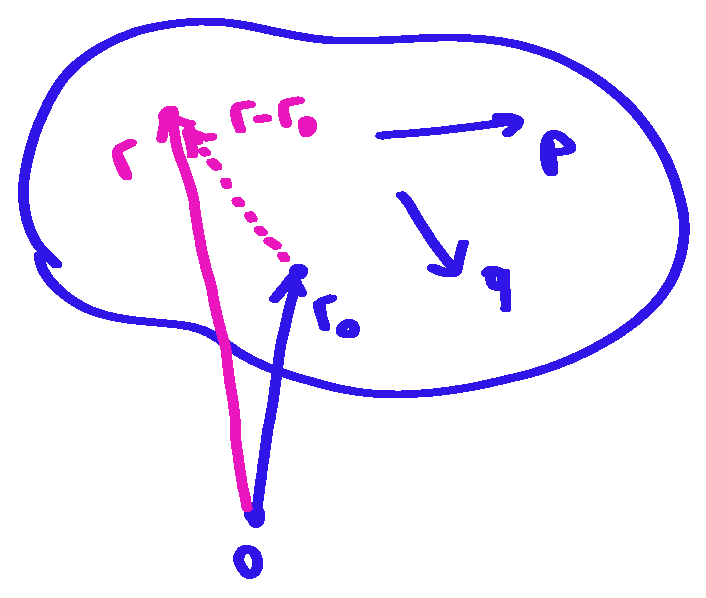
\includegraphics[width=0.5\textwidth]{dot-and-two-vectors-on-the-plane}
    
    \caption{Два направляющих вектора $\bds p$ и $\bds q$, таких что $\bds p \hm{\not\parallel} \bds q$, и начальная точка $\bds r_0$ однозначно задают плоскость.}
    \label{fig:dot-and-two-vectors-on-the-plane}
  \end{figure}
  
  Одно векторное уравнение равносильно системе из трёх скалярных уравнений:
  \[
    \left\{
      \begin{aligned}
        &x = x_0 + t_1 p_x + t_2 q_x\\
        &y = y_0 + t_1 p_y + t_2 q_y\\
        &z = z_0 + t_1 p_z + t_2 q_z
      \end{aligned}
    \right.
  \]
  где введены обозначения $x, y, z$ для компонент $\bds r$; $x_0, y_0, z_0$ для компонент $\bds r_0$; и $p_x, p_y, p_z$ и $q_x, q_y, q_z$ для компонент векторов $\bds p$ и $\bds q$ соответственно.
  
  Ещё один вариант переписать уравнение (\ref{eq:plane-vector-parametric}) исходит из того, что векторы $\bds r \hm- \bds r_0$, $\bds p$ и $\bds q$ компланарны.
  То есть объём параллелепипеда, построенного на них, равен нулю.
  То есть:
  \[
    \boxed{
      (\bds r - \bds r_0, \bds p, \bds q) = 0
    }
  \]
  
  Как и для прямой на плоскости, для плоскости в пространстве, из аналогичных рассуждений, можно выписать \emph{нормальное векторное уравнение}:
  \begin{equation}\label{eq:plane-normal}
    \boxed{(\bds r - \bds r_0, \bds n) = 0}
  \end{equation}
  \[
    (\bds r, \bds n) = D,\quad D \in \RR
  \]
  где $\bds n$~---~нормальный вектор плоскости, то есть вектор, перпендикулярный плоскости.
  
  От нормального векторного уравнения можно перейти к ``популярной задачке'' на нахождение расстояния от точки до плоскости.
  Пусть есть точка $M(x, y)$ и плоскость $\alpha$, заданная нормальным векторным уравнением (\ref{eq:plane-normal}).
  Тогда расстояние $\rho(M, \alpha)$, находится точно так же, как в прошлый раз для случая точки и прямой:
  \begin{equation}\label{eq:distance-from-point-to-plane}
    \rho(M, \alpha) = \left|\frac{(\bds r - \bds r_0, \bds n)}{|\bds n|}\right|
  \end{equation}
  
  Если система координат декартова прямоугольная (ПДСК) и известно уравнение плоскости $\alpha$ в виде (\ref{eq:plane-by-coords}), то, точно так же, как и в прошлый раз, формула для вычисления расстояния преобразуется в следующую:
  \[
    \rho(M, \alpha) = \frac{|A x_0 + B y_0 + C z_0 + D|}{\sqrt{A^2 + B^2 + C^2}}
  \]
  
  Зададимся теперь вопросом о связи разных представлений одной и той же плоскости в пространстве.
  Так, если, например, известно уравнение плоскости вида~(\ref{eq:plane-by-coords}), то как из него получить направляющие векторы, необходимые, например, для уравнения~(\ref{eq:plane-vector-parametric})?
  Это можно сделать так же, как в прошлый раз для прямой.
  Пусть есть две различные точки на плоскости: $P(x_1, y_1)$ и $Q(x_2, y_2)$.
  Тогда направляющий вектор можно выбрать в виде $\vv{PQ} \hm= (x_2 \hm- x_1, y_2 \hm- y_1)$.
  Запишем, что значит, что точки $P$ и $Q$ лежат на плоскости~---~их координаты удовлетворяют уравнению плоскости:
  \[
    \left\{
      \begin{aligned}
        &A x_1 + B y_1 + C z_1 + D = 0\\
        &A x_2 + B y_2 + C z_2 + D = 0
      \end{aligned}
    \right.
  \]
  
  Нам нужны разности координат~---~тогда вычтем из второго уравнения первое.
  Получим:
  \[
    A(x_2 - x_1) + B(y_2 - y_1) + C(z_2 - z_1) = 0
  \]
  
  Но нам не нужны сами точки $P$ и $Q$.
  Мы хотим найти только направляющий вектор плоскости.
  Допустим, у искомого направляющего вектора координаты $(\alpha, \beta, \gamma)$.
  Тогда для поиска этих координат можно использовать уравнение:
  \begin{equation}\label{eq:search-for-napravlayushii}
    \boxed{
      A \alpha + B \beta + C \gamma = 0
    }
  \end{equation}
  
  По виду это уравнение напоминает полученное в прошлый раз для поиска компонент направляющего вектора прямой (что в принципе не удивительно, ведь рассуждения были проведены те же самые).
  В прошлый раз получилось довольно быстро подобрать направляющий вектор прямой~---~подошёл вектор вида $(-B, A)$.
  Здесь же... всё уже не так очевидно, поэтому обычно направляющие векторы плоскости ищут отдельно в каждой конкретной задаче, просто ``внимательно вглядываясь'' в соотношение (\ref{eq:search-for-napravlayushii}).
  Но вообще... можно попытаться найти направляющие векторы и в общем виде.
  Сделаем же это (почему бы и нет)!
  
  (...Внимательно смотрим на (\ref{eq:search-for-napravlayushii}), при этом понимая, что хотя бы одна компонента у направляющего вектора обязана быть отлична от нуля.)
  
  Не сложно видеть, что направляющие векторы плоскости могут быть выбраны в общем случае как следующие векторы:
  \begin{equation}\label{eq:two-vectors-for-plane-in-general}
    \bds p = \begin{pmatrix}
      B + C\\
      -A - C\\
      -A + B
    \end{pmatrix},
    \quad \bds q = \begin{pmatrix}
      B - C\\
      -A + C\\
      A - B
    \end{pmatrix}
  \end{equation}
  
  Но запоминать эти формулы не стоит)
  Проще каждый раз ``подбирать''.
  
  \bigskip
  
  Теперь вернёмся ещё раз к прямой.
  Как на прямую ``можно смотреть'' в пространстве?
  Векторное параметрическое уравнение
  \begin{equation}\label{eq:line-vector-parametric}
    \boxed{\bds r = \bds r_0 + \bds a t,\quad t \in \RR}
  \end{equation}
  и в пространстве, очевидно, описывает прямую (``сдвиг в $\bds r_0$'', а потом ``сдвиг вдоль $\bds a$'').
  Правда, в скалярном виде получается система из \emph{трёх} уравнений:
  \[
    \left\{
      \begin{aligned}
        &x = x_0 + a_x t\\
        &y = y_0 + a_y t\\
        &z = z_0 + a_z t
      \end{aligned}
    \right.
  \]
  
  Выражая из каждого уравнения системы параметр $t$ и приравнивая, получаем \emph{каноническое уравнение прямой в пространстве}:
  \[
    \frac{x - x_0}{a_x} = \frac{y - y_0}{a_y} = \frac{z - z_0}{a_z}
  \]
  
  Уравнение (\ref{eq:line-vector-parametric}) фактически говорит о том, что для точек прямой и только для них верно, что $\bds r - \bds r_0 \hm\parallel \bds a$.
  В пространстве условие коллинеарности двух векторов можно записать таким образом:
  \[
    [\bds r - \bds r_0, \bds a] = \bds 0
  \]
  \[
    [\bds r, \bds a] = \bds b
  \]
  
  В пространстве также появляется ещё один, совершенно новый, способ описать прямую.
  Как пересечение двух непараллельных плоскостей (\ref{fig:two-planes-have-something-in-common}):
  \begin{equation}\label{eq:line-as-plane-intersection}
    \boxed{
      \left\{
        \begin{aligned}
          &A_1 x + B_1 y + C_1 z + D_1 = 0\\
          &A_2 x + B_2 y + C_2 z + D_2 = 0
        \end{aligned}
      \right.
    }
  \end{equation}
  
  \begin{figure}[h]
    \centering
    
    \includegraphics[width=0.3\textwidth]{two-planes-have-something-in-common}
    
    \caption{Две непараллельных плоскости пересекаются по прямой.}
    \label{fig:two-planes-have-something-in-common}
  \end{figure}
  
  
  \section{Задачи}
  
  Последний рассмотренный сюжет (про прямую как пересечение плоскостей) плавно перетекает в номер
  
  \subsection{\# 6.15}
  
  \begin{problem}
    Доказать, что направляющий вектор $\bds a$ прямой, заданной системой (\ref{eq:line-as-plane-intersection}), может быть найден по формуле\footnote{В общей декартовой системе это \textbf{не} векторное произведение. На формулу надо смотреть именно так, как она написана: определитель некоторой матрицы.}:
    \begin{equation}\label{eq:parallel-for-line-as-intersection}
      \boxed{
        \bds a = \begin{vmatrix}
          \bds e_1 & \bds e_2 & \bds e_3\\
          A_1      & B_1      & C_1\\
          A_2      & B_2      & C_2
        \end{vmatrix}
      }
    \end{equation}
  \end{problem}
  
  \begin{solution}
    Распишем компоненты вектора:
    \[
      \bds a = \bigl\{
        \textcolor{my-green}{B_1} \textcolor{my-blue}{C_2} - \textcolor{my-green}{C_1} \textcolor{my-blue}{B_2},
        \textcolor{my-green}{C_1} \textcolor{my-blue}{A_2} - \textcolor{my-green}{A_1} \textcolor{my-blue}{C_2},
        \textcolor{my-green}{A_1} \textcolor{my-blue}{B_2} - \textcolor{my-green}{B_1} \textcolor{my-blue}{A_2}
      \bigr\}
    \]
    
    Можно теперь просто подставить эти компоненты в соотношения (\ref{eq:search-for-napravlayushii}), выписанные для обеих плоскостей, и убедиться, что $\bds a$ в самом деле им обеим параллелен.
    А значит, параллелен и прямой, по которой плоскости пересекаются.
    То есть может быть выбран её направляющим вектором.
    
    Проверить было несложно.
    Сложнее... понять, как вообще дошли до того, чтобы искать $\bds a$ в описанном виде)
    Некоторую интуицию за всем этим можно подметить из того, что ``разности'' между коэффициентами, соответствующими одной и той же плоскости, стоят в компонентах $\bds a$ в целом так же, по ``такой же схеме'', как мы получили в (\ref{eq:two-vectors-for-plane-in-general})...
  \end{solution}
  
  
  \subsection{\# 6.3}
  
  \begin{problem}
    Выписать необходимое и достаточное условие, при котором прямые
    $
      l_1\colon \bds r \hm= \bds r_1 \hm+ \bds a_1 t
    $ и
    $
      l_2\colon \bds r \hm= \bds r_2 \hm+ \bds a_2 t
    $
    \begin{itemize}
      \item пересекаются в одной точке
      \item скрещиваются
      \item параллельны, но не совпадают
      \item совпадают
    \end{itemize}
  \end{problem}
  
  \begin{solution}
    \begin{figure}[h]
      \centering
      
      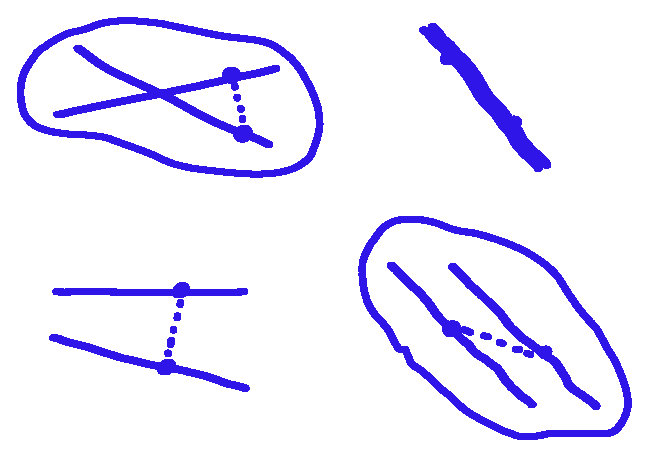
\includegraphics[width=0.5\textwidth]{different-cases}
      
      \caption{Возможные случаи взаимного расположения двух прямых в пространстве.}
      \label{fig:different-cases}
    \end{figure}
  
    Для пересечения надо потребовать $\bds a_1 \not\parallel \bds a_2$ (\ref{fig:different-cases}).
    
    На плоскости этого было достаточно.
    В пространстве же это условие подходит ещё и для скрещивания.
    Надо как-то ``разделить'' пересечение и скрещивание.
    Прямые скрещиваются, если не лежат в одной плоскости.
    Отсюда можно заметить, что для скрещивающихся прямых векторы $\bds r_2 \hm- \bds r_1$, $\bds a_1$ и $\bds a_2$ будут некомпланарны.
    И наоборот: если указанные векторы компланарны, то прямые будут лежать в одной плоскости.
    Итого, условие скрещивания:
    \[
      \left\{
        \begin{aligned}
          &[\bds a_1, \bds a_2] \not= \bds 0\\
          &(\bds r_2 - \bds r_1, \bds a_1, \bds a_2) \not= 0
        \end{aligned}
      \right.
    \]
    где воспользовались тем, что условие $\bds a_1 \not\parallel \bds a_2$ можно переписать в пространстве как $[\bds a_1, \bds a_2] \hm{\not=} \bds 0$.
    
    Пересечение в одной точке определяется такими условиями:
    \[
      \left\{
        \begin{aligned}
          &[\bds a_1, \bds a_2] \not= \bds 0\\
          &(\bds r_2 - \bds r_1, \bds a_1, \bds a_2) = 0
        \end{aligned}
      \right.
    \]
    
    Чтобы перейти к следующим случаям взаимного расположения прямых в пространстве (параллельность и совпадение), можно сразу обратить условие неколлинеарности направляющих векторов.
    То есть в оставшихся случаях имеем $[\bds a_1, \bds a_2] \hm= \bds 0$.
    На самом деле мы уже как бы перешли в плоскость, а с плоскостью уже разобрались в прошлый раз.
    Поэтому можно сразу написать, что параллельность, но не совпадение~---~это
    \[
      \left\{
        \begin{aligned}
          &[\bds a_1, \bds a_2] = \bds 0\\
          &[\bds r_2 - \bds r_1, \bds a_1] \not= \bds 0
        \end{aligned}
      \right.
    \]
    
    И совпадение:
    \[
      \left\{
        \begin{aligned}
          &[\bds a_1, \bds a_2] = \bds 0\\
          &[\bds r_2 - \bds r_1, \bds a_1] = \bds 0
        \end{aligned}
      \right.
    \]
  \end{solution}
  
  
  
  \subsection{\# 6.10(1)}
  
  \begin{problem}
    Составить уравнение проекции $l'$ прямой $l\colon \bds r \hm= \bds r_0 \hm+ \bds a t$ $(t \hm\in \RR)$, не перпендикулярной плоскости $\alpha\colon (\bds r, \bds n) \hm= D$, на эту плоскость.
  \end{problem}
  
  \begin{solution}
    % TODO: pic
    
    Раз прямая $l$ и плоскость $\alpha$ не перпендикулярны, то проекцией $l$ на $\alpha$ также будет прямая (а не точка).
    
    \medskip
    
    \emph{Случай 1: пересечение}.
    Допустим, прямая $l$ и плоскость $\alpha$ пересекаются в некоторой точке $M(\bds r_1)$ (см. рисунок~\ref{fig:project-line-when-intersect}).
    Найдём её:
    \[
      \left\{
        \begin{aligned}
          &\bds r_1 = \bds r_0 + \bds a t_1\\
          &(\bds r_1, \bds n) = D
        \end{aligned}
      \right.
    \]
    \[
      (\bds r_0 + \bds a t_1, \bds n) = D \Rightarrow t_1 = \frac{D - (\bds r_0, \bds n)}{(\bds a, \bds n)}
    \]
    
    \begin{figure}[h]
      \centering
      
      \includegraphics[width=0.5\textwidth]{project-line-when-intersect}
      
      \caption{Проекция прямой на плоскость в случае пересечения прямой и плоскости.}
      \label{fig:project-line-when-intersect}
    \end{figure}
    
    Чем определяется прямая $l'$?
    Точка $M$ принадлежит также и $l'$.
    Таким образом, для ``полного понимания'' $l'$ не хватает только направляющего вектора.
    Но его можно найти, зная направляющий вектор $\bds a$ прямой $l$.
    Действительно, упомянутый $\bds a$ можно представить как сумму двух векторов: $\bds a_n$, параллельного $\bds n$, и $\bds a_{\alpha}$, перпендикулярного ему (то есть лежащего в плоскости $\alpha$):
    \[
      \bds a = \bds a_n + \bds a_{\alpha},\quad \bds a_n \parallel \bds n, \bds a_{\alpha} \perp \bds n
    \]
    
    Но составляющая $\bds a_{\alpha}$~---~и есть направляющий вектор $l'$:
    \[
      \bds a_{\alpha} = \bds a - \frac{(\bds a, \bds n)}{|\bds n|^2} \bds n
    \]
    
    И тогда уравнение прямой $l'$:
    \[
      \bds r = \bds r_1 + \bds a_{\alpha} t,\quad t \in \RR
    \]
    
    \medskip
    
    \emph{Случай 2: нет пересечения}.
    Но возможен и такой случай, когда прямая $l$ \emph{параллельна} плоскости $\alpha$ (\ref{fig:project-line-when-no-intersect}).
    В этом случае уже нет никакой ``особой'' точки, за которую можно бы было ``зацепиться''.
    Но можно... просто взять некоторую случайную точку с прямой $l$ и спроецировать её на $\alpha$.
    Получим точку с $l'$.
    А направляющий вектор $l'$ будем таким же, как у~$l$.
    
    \begin{figure}[h]
      \centering
      
      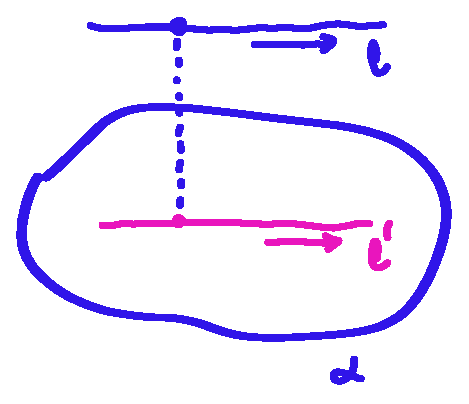
\includegraphics[width=0.5\textwidth]{project-line-when-no-intersect}
      
      \caption{Проекция прямой на плоскость в случае, когда прямая и плоскость не пересекаются.}
      \label{fig:project-line-when-no-intersect}
    \end{figure}
    
    Спроецируем на $\alpha$ точку $\bds r_0$.
    Пусть радиус-вектор ортогональной проекции есть $\bds r_0'$.
    Тогда условия, однозначно задающие $\bds r_0'$:
    \[
      \left\{
        \begin{aligned}
          &(\bds r_0 - \bds r_0') \parallel \bds n\\
          &\bds r_0' \in \alpha
        \end{aligned}
      \right. \Leftrightarrow
      \left\{
        \begin{aligned}
          &\bds r_0 - \bds r_0' = k \bds n\\
          &(\bds r_0', \bds n) = D
        \end{aligned}
      \right.
    \]
    \[
      (\bds r_0 - k \bds n, \bds n) = D \Rightarrow k = \frac{(\bds r_0, \bds n) - D}{|\bds n|^2}
    \]
    
    Уравнение проекции $l'$:
    \[
      \bds r = \bds r_0' + \bds a t,\quad t \in \RR
    \]
  \end{solution}
  
  
  
  \subsection{\# 6.10(4) + \# 6.11(8)}
  
  \begin{problem}
    Составить уравнение прямой, пересекающей две скрещивающиеся прямые
    \[
      l_1\colon \bds r = \bds r_1 + \bds a_1 t
    \]
    \[
      l_2\colon \bds r = \bds r_2 + \bds a_2 t
    \]
    под прямыми углами (общий перпендикуляр к скрещивающимся прямым).
    Найти расстояние между прямыми $l_1$ и $l_2$.
  \end{problem}
  
  \begin{solution}
    \leavevmode
    
    \emph{Способ 1: ``понятный, но долгий''}.
    Пусть прямая~--~общий перпендикуляр пересекает прямые $l_1$ и $l_2$ в точках $P(\bds r_p)$ и $Q(\bds r_q)$ соответственно.
    Эти точки можно найти.
    Они однозначно определяются следующим набором условий:
    \[
      \left\{
        \begin{aligned}
          &P \in l_1\\
          &Q \in l_2\\
          &\vv{PQ} \perp \bds a_1\\
          &\vv{PQ} \perp \bds a_2
        \end{aligned}
      \right.
      \Leftrightarrow \left\{
        \begin{aligned}
          &\bds r_p = \bds r_1 + \bds a_1 t_p\\
          &\bds r_q = \bds r_2 + \bds a_2 t_q\\
          &(\bds r_q - \bds r_p, \bds a_1) = 0\\
          &(\bds r_q - \bds r_p, \bds a_2) = 0
        \end{aligned}
      \right.
    \]
    
    При подстановке $\bds r_p$ и $\bds r_q$ из первого и второго уравнений в третье и четвёртое, получаем систему линейных уравнений $2 \hm\times 2$ относительно $t_p$ и $t_q$.
    Её точно можно будет решить (в процессе решения должно будет ``вылезти'' условие того, что прямые должны скрещиваться).
    Найдя $t_p$ и $t_q$, можно будет вычислить $\bds r_p$ и $\bds r_q$.
    А далее можно уже получить и уравнение общего перпендикуляра (на тот момент будем знать и начальную точку, и направляющий вектор), и длину $PQ \hm= |\bds r_q \hm- \bds r_p|$~---~расстояние между прямыми $l_1$ и $l_2$.
    Но... есть способ решения покороче.
    
    \medskip
    
    \emph{Способ 2 (перпендикуляр): ``непонятный, но покороче'', или ``а так вообще... можно?..''}
    Найдём уравнение общего перпендикуляра как прямой, являющейся пересечением двух плоскостей $\alpha$ и $\beta$ (\ref{fig:skew-alpha-beta}).
    Первая плоскость $\alpha$ проходит через прямую $l_1$ и общий перпендикуляр.
    Вторая плоскость $\beta$ проходит через прямую $l_2$ и общий перпендикуляр.
    (Очевидно, плоскости $\alpha$ и $\beta$ пересекаются по искомому перпендикуляру.)
    Какие уравнения описывают указанные плоскости?
    
    \begin{figure}[h]
      \centering
      
      \includegraphics[width=0.5\textwidth]{skew-alpha-beta}
      
      \caption{К поиску общего перпендикуляра к двум скрещивающимся прямым.}
      \label{fig:skew-alpha-beta}
    \end{figure}
    
    Ещё раз посмотрим на $\alpha$.
    Раз $l_1 \hm\subset \alpha$, то и точка с радиусом-вектором $\bds r_1$ (начальная точка прямой $l_1$) лежит на $\alpha$.
    В то же время $\bds a_1$ и направляющий вектор общего перпендикуляра будут направляющими векторами плоскости $\alpha$ (неколлинеарными).
    Направляющий вектор общего перпендикуляра можно выбрать как $[\bds a_1, \bds a_2]$.
    Таким образом, для точки плоскости $\alpha$ с радиусом-вектором $\bds r$ и только для такой точки верно, что векторы $\bds r \hm- \bds r_1$, $\bds a_1$, $[\bds a_1, \bds a_2]$ оказываются компланарны.
    Аналогично, компланарны будут векторы $\bds r \hm- \bds r_2$, $\bds a_2$ и $[\bds a_1, \bds a_2]$ для любой точки с радиусом-вектором $\bds r$ на плоскости $\beta$.
    Объединяя уравнения описанных плоскостей в систему, получаем... ``уравнение'' общего перпендикуляра:
    \[
      \left\{
        \begin{aligned}
          &(\bds r - \bds r_1, \bds a_1, [\bds a_1, \bds a_2]) = 0\\
          &(\bds r - \bds r_2, \bds a_2, [\bds a_1, \bds a_2]) = 0
        \end{aligned}
      \right.
    \]
    
    \medskip
    
    \emph{Способ 2 (расстояние)}.
    
    Перейдём к вопросу о расстоянии между скрещивающимися прямыми.
    Один возможный вариант решения уже разобрали (через поиск радиусов-векторов $\bds r_p$ и $\bds r_q$).
    Рассмотрим ещё один несложный способ.
    
    \begin{figure}[h]
      \centering
      
      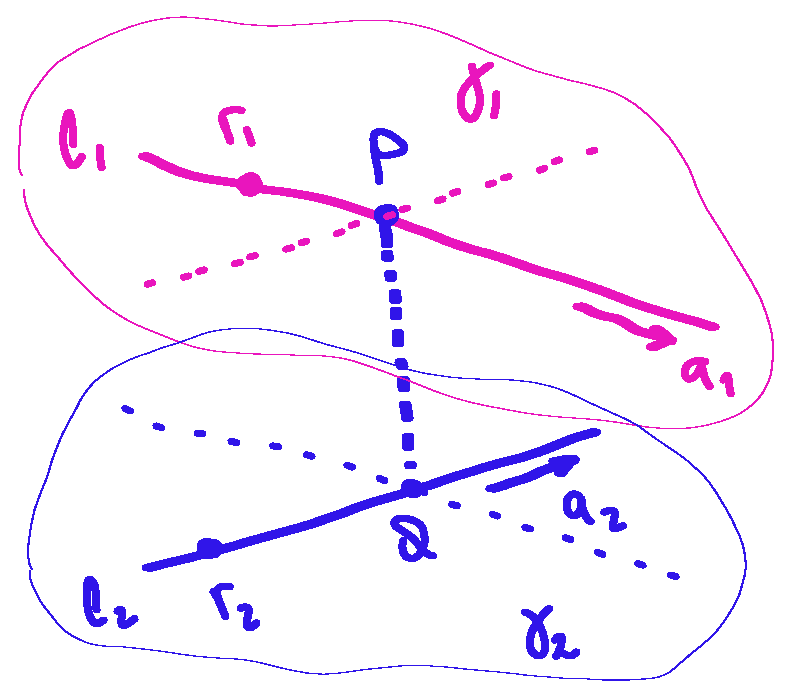
\includegraphics[width=0.5\textwidth]{skew-gamma1-gamma2}
      
      \caption{К поиску расстояния между скрещивающимися прямыми.}
      \label{fig:skew-gamma1-gamma2}
    \end{figure}
    
    Перенесём параллельно прямую $l_2$ до пересечения с $l_1$.
    Получим плоскость $\gamma_1$, проходящую через $l_1$ и параллельную также $l_2$ (\ref{fig:skew-gamma1-gamma2}).
    Перенесём также параллельно $l_1$ до пересечения с $l_2$, получим плоскость $\gamma_2$.
    Не сложно видеть, что расстояние между $l_1$ и $l_2$ есть расстояние между $\gamma_1$ и $\gamma_2$.
    Которое равно расстоянию от некоторой точки плоскости $\gamma_2$ (например, точки $\bds r_2$) до плоскости $\gamma_1$.
    Но это просто ``расстояние от точки до плоскости'', которое можно посчитать по формуле (\ref{eq:distance-from-point-to-plane}).
    При этом точка, от которой считаем расстояние~---~это $\bds r_2$; начальная точка плоскости $\gamma_1$~---~это $\bds r_1$; а вектор нормали к плоскости $\gamma_1$ можно взять как $[\bds a_1, \bds a_2]$:
    \[
      \rho(l_1, l_2) = \left|\frac{(\bds r_2 - \bds r_1, [\bds a_1, \bds a_2])}{|[\bds a_1, \bds a_2]|}\right|
    \]
    
    Если посмотреть теперь внимательнее на полученную формулу, то можно увидеть за ней ещё такой смысл.
    Искомое расстояние~---~это высота параллелепипеда, построенного на векторах $(\bds r_2 \hm- \bds r_1)$, $\bds a_1$ и $\bds a_2$.
    Высота, проведённая к основанию, соответствующему векторам $\bds a_1$ и $\bds a_2$.
  \end{solution}
  
  
  
  \subsection{\# 6.18(1)}
  
  \begin{problem}
    Составить уравнение прямой $l$, проходящей через точку $A(1, 3, 1)$ и параллельной прямой $l_2$, заданной как пересечение плоскостей:
    \[
      l_2\colon \left\{
        \begin{aligned}
          &\hphantom{2}x + \hphantom{3}y - z + 2 = 0\\
          &2x            + 3y            + z \hphantom{+ 2} = 0
        \end{aligned}
      \right.
    \]
  \end{problem}
  
  \begin{solution}
    Уже дана начальная точка $\bds r_0$ прямой $l$.
    Не хватает только, например, направляющего вектора.
    Который, очевидно, надо искать из условия параллельности $l$ и $l_2$.
    
    Раз прямые параллельны, то в качестве направляющего $l$ можно взять направляющий $l_2$.
    Его же можно найти по формуле (\ref{eq:parallel-for-line-as-intersection}):
    \[
      \bds a = \begin{vmatrix}
        \bds e_1 & \bds e_2 & \bds e_3\\
        1        & 1        & -1\\
        2        & 3        & 1
      \end{vmatrix}
      = (4, -3, 1)
    \]
    
    Итого, уравнение прямой $l$:
    \[
      \bds r = \bds r_0 + \bds a t
    \]
    
    Расписывая в координатах:
    \[
      \begin{pmatrix}
        x \\ y \\ z
      \end{pmatrix}
      = \begin{pmatrix}
        1 \\ 3 \\ 1
      \end{pmatrix}
      + \begin{pmatrix}
        4 \\ -3 \\ 1
      \end{pmatrix} t,\quad t \in \RR
    \]
    
    Или в каноническом виде:
    \[
      \frac{x - 1}{4} = \frac{y - 3}{-3} = \frac{z - 1}{1}
    \]
  \end{solution}
  
  
  \subsection{\# 6.17(1)}
  
  \begin{problem}
    Составить уравнение плоскости $\alpha$, проходящей через точку $A(1, -1, 2)$ и параллельной плоскости $\alpha_2$, заданной уравнением в общей декартовой системе координат:
    \[
      \alpha_2\colon x - 3y + 2z + 1 = 0
    \]
  \end{problem}
  
  \begin{solution}
    Раз плоскости параллельны, то должны быть пропорциональны коэффициенты $A$, $B$, $C$ в их уравнениях вида (\ref{eq:plane-by-coords}).
    Почему так~---~можно понять из такого наблюдения.
    Если известен нормальный вектор плоскости $\bds n$, то её можно описать уравнением:
    \[
      (\bds r - \bds r_0, \bds n) = 0
    \]
    
    Разложим радиус-вектор точки плоскости $\bds r$ по базису:
    \[
      \bds r = x \bds e_1 + y \bds e_2 + z \bds e_3
    \]
    
    Теперь подставим в нормальное уравнение плоскости:
    \[
      (\bds e_1, \bds n) x + (\bds e_2, \bds n) y + (\bds e_3, \bds n) z - (\bds r_0, \bds n) = 0
    \]
    
    Видно, что в общей декартовой системе координат коэффициенты $A$, $B$, $C$~---~не компоненты вектора нормали, а скалярные произведения вида $(\bds e_i, \bds n)$.
    Но в любом случае коэффициенты пропорциональны компонентам вектора $\bds n$.
    
    Если же плоскости параллельны, то вектора нормали для них можно выбрать одинаковыми.
    Что и даст вообще одинаковые коэффициенты $A$, $B$, $C$.
    В общем случае у параллельных плоскостей нормали параллельны, поэтому коэффициенты перед переменными в уравнении должны быть пропорциональны.
    
    Итак, уравнение плоскости $\alpha$ можно искать в виде:
    \[
      x - 3y + 2z + D = 0
    \]
    
    Подставляя координаты точки $A$, находим $D$:
    \[
      1 - 3 \cdot (-1) + 2 \cdot 2 + D = 0 \Rightarrow D = -8
    \]
    
    Итоговое уравнение:
    \[
      x - 3y + 2z - 8 = 0
    \]
  \end{solution}
  
  % Неплохой номер, но в конспект можно и не включать...
  %
  %\subsection{\# 6.25(5)}
  %
  %\begin{problem}
  %\end{problem}
  %
  %\begin{solution}
  %\end{solution}
\end{document}
